\begin{figure*}[t]
  \centering
  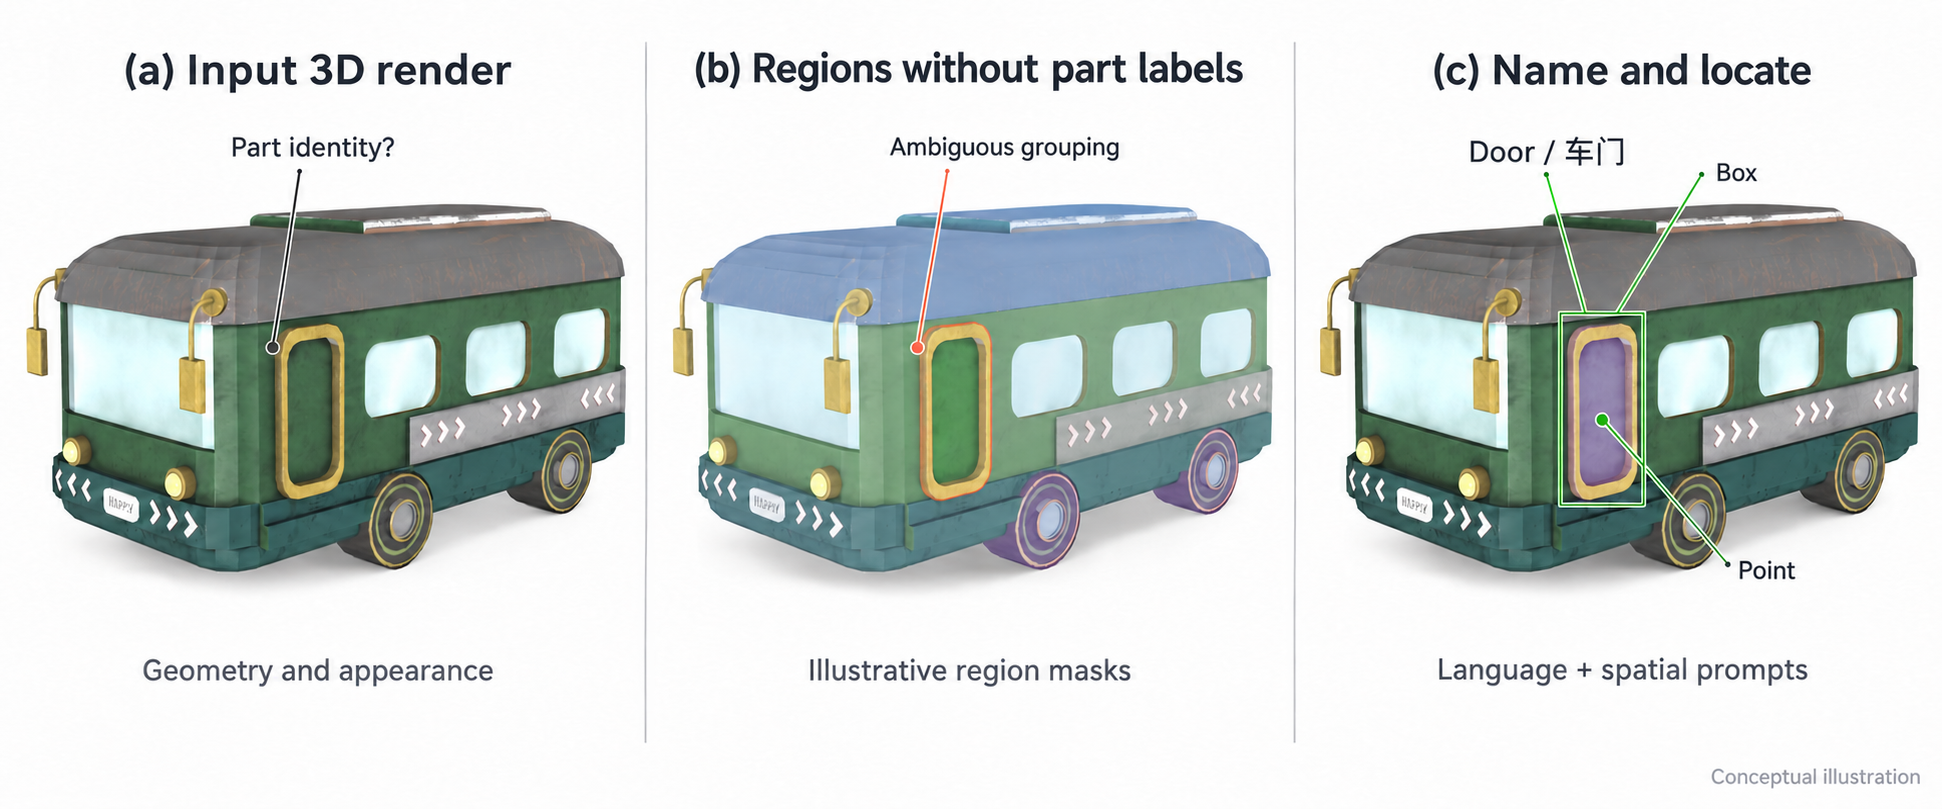
\includegraphics[width=\textwidth]{images/fig3_motivation.png}
  \caption{研究动机的概念示意。（a）三维渲染提供几何与外观，却未必提供可查询的部件名称；（b）无语义区域划分不能直接回答某一区域对应什么部件；（c）视觉语言模型将名称与框、点等空间提示关联，使分割目标具有明确的语义指向。该图为概念插图，不是 B/C 的实测对比，也不用于证明分割精度优越。}
  \label{fig:motivation}
\end{figure*}
